
A pendulum is a rigid body that can swing under the influence of gravity. It is attached at the top so it can roatate freely in a two-dimensional plane ($x,y$).
We will assume a thin rectangular shape with the mass equally distributed. A double pendulum is a pendulum connected to the end of another pendulum. Contrary to the 
regular movement of a pendulum, the motion of a double-pendulum is very irregular when sufficient energy is put into the system. 

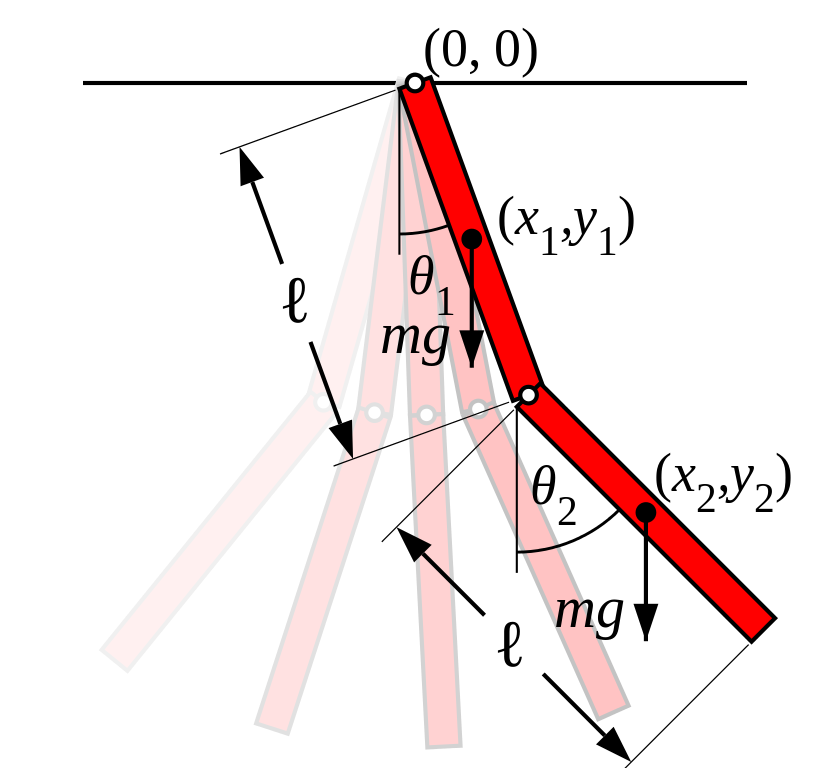
\includegraphics[height=4cm]{Double-compound-pendulum.png}

The dynamics of a double-pendulum can be descibed with the following equations 
( This example was copied from https://en.wikipedia.org/wiki/Double\_pendulum )

variables $\theta_1, \theta_2, p_{\theta_1}, p_{\theta_2}$:
\begin{eqnarray}
   \frac{d \theta_1}{dt}= \frac{6}{m l^2} \frac{2 p_{\theta_1} - 3cos(\theta_1-\theta_2) p_{\theta_2}}
   {16-9 cos^2(\theta_1-\theta_2)}\\
   \frac{d \theta_2}{dt}= \frac{6}{m l^2} \frac{8 p_{\theta_2} - 3cos(\theta_1-\theta_2) p_{\theta_1}}
   {16-9 cos^2(\theta_1-\theta_2)}\\
   \frac{dp_{\theta_1}}{dt} = -\frac{1}{2} ml^2 \left( \frac{d \theta_1}{dt} \frac{d \theta_2}{dt} sin(\theta_1-\theta_2) + 3\frac{g}{l} sin(\theta_1) \right)  \\
   \frac{dp_{\theta_1}}{dt} = -\frac{1}{2} ml^2 \left( -\frac{d \theta_1}{dt} \frac{d \theta_2}{dt} sin(\theta_1-\theta_2) + \frac{g}{l} sin(\theta_2) \right) 
\end{eqnarray}
where the $x,y$-position of the middle of the two segments can be computed as:
\begin{eqnarray}
   x_1 = \frac{l}{2} sin(theta_1) \\
   y_1 = \frac{-l}{2} cos(\theta_1) \\
   x_2 = l ( sin(\theta_1) + \frac{1}{2} sin(\theta_2) )
   y_2 = -l ( cos(\theta_1) + \frac{1}{2} cos(\theta_2) )
\end{eqnarray}

This model, although simple, is very nonlinear and has a chaotic nature.  Its
solution is very sensitive to the parameters and the initial conditions: a
small difference in those values can lead to a very different solution.

The purpose of this exercise is to get you started with OpenDA. You will learn
to run a model in OpenDA, make modifications to the input files and plot the
results.

\begin{itemize}
\item The input for this exercise is located in directory {\tt Exercise\_1}.
      For Linux and Mac OS X, go to this directory and start {\tt oda\_run.sh}, the
      main application of OpenDA. For Windows, start the main application with 
      {\tt oda\_run\_gui.bat} from the {\tt \$OPENDA/bin} directory. The main 
      application allows you to view and edit the OpenDA configuration files, run your
      simulations and visualize the results.
\item Try to run a simulation with the Lorenz model. You can use the
      configuration file {\tt simulation\_unperturbed.oda}. The results are
      written to {\tt simulation\_unperturbed\_results.m}, You can make a
      plot using Octave or Matlab. Load the results using the function
      {\tt load\_results}:
      \begin{lstlisting}[language=Matlab,frame=single,caption={Matlab}]
       [t,xyz,tobs,obs]=load_results('simulation_unperturbed_results');
       plot3(xyz(1,:),xyz(2,:),xyz(3,:));
       grid on;
      \end{lstlisting}
      Or with python. To run the examples you need python 2.7 with the packages numpy and matplotlib installed. Depending
      on your environment you may need to import these packages.
      \begin{lstlisting}[language=Python,frame=single,caption={Python initialize}]
      import numpy as np
      import matplotlib.pyplot as plt
      \end{lstlisting}
      and next make the plot
      \begin{lstlisting}[language=Python,frame=single,caption={Python}]
      #load data
      import simulation_unperturbed_results as sim
      # make 3d line plot
      from mpl_toolkits.mplot3d import Axes3D
      fig1 = plt.figure()
      ax = fig1.add_subplot(111, projection='3d')
      # note we start counting at 0 now
      Axes3D.plot(ax,sim.x[:,0],sim.x[:,1],sim.x[:,2])
      \end{lstlisting}
      
      Now make a plot of only the first variable of the model ({\tt xyz(1,:)}).
      \begin{lstlisting}[language=Matlab,frame=single,caption={Matlab}]
      plot(t,xyz(1,:),'b')
      \end{lstlisting}
      \begin{lstlisting}[language=Python,frame=single,caption={Python}]
      plt.figure()
      plt.plot(sim.model_time,sim.x[:,0],'b')
      plt.show()
      \end{lstlisting}
%

\item Observations of the first variable are available as well. Make a plot of
      the observations together with the simulation results.
      \begin{lstlisting}[language=Matlab,frame=single,caption={Matlab}]
      [t,xyz,tobs,obs]=load_results('simulation_unperturbed_results');
       plot(t,xyz(1,:),'b')
       hold on
       plot(tobs,obs,'r*');
       hold off
      \end{lstlisting}
      \begin{lstlisting}[language=Python,frame=single,caption={Python}]
      import simulation_unperturbed_results as sim
      plt.plot(sim.model_time,sim.x[:,0])
      plt.plot(sim.analysis_time,sim.obs,'r*')
      \end{lstlisting}

\item Then you can start an alternative simulation with the lorenz model that
       starts with a slightly different initial condition using the
       configuration file {\tt simulation\_perturbed.oda} that starts with
       slightly different initial conditions.

\item  Visualize the unperturbed and perturbed results in a single plot. Make
       a 3d trajectory plot and a 2d plot in time of first variable. Do you see
       the solutions diverging like the theory predicts?
      \begin{lstlisting}[language=Matlab,frame=single,caption={Matlab}]
       [t1,xyz1,tobs1,obs1]=load_results('simulation_unperturbed_results');
       [t2,xyz2,tobs2,obs2]=load_results('simulation_perturbed_results');
       figure(1)
       plot3(xyz1(1,:),xyz1(2,:),xyz1(3,:),'b');
       hold on
       plot3(xyz2(1,:),xyz2(2,:),xyz2(3,:),'r');
       hold off
       legend('unperturbed','perturbed')

       figure(2)
       plot(t1,xyz1(1,:),'b')
       hold on
       plot(t2,xyz2(1,:),'r')
       hold off
       legend('unperturbed','perturbed')
      \end{lstlisting}
      \begin{lstlisting}[language=Python,frame=single,caption={Python}]
      #load unperturbed and perturbed results
      import simulation_unperturbed_results as sim
      import simulation_perturbed_results as simp
      fig3 = plt.figure()
      ax = fig3.add_subplot(111, projection='3d')
      Axes3D.plot(ax,sim.x[:,0],sim.x[:,1],sim.x[:,2],'b')
      Axes3D.plot(ax,simp.x[:,0],simp.x[:,1],simp.x[:,2],'r')

      fig4 = plt.figure()
      plt.plot(sim.model_time,sim.x[:,0],'b')
      plt.plot(simp.model_time,simp.x[:,0],'r')
      \end{lstlisting}

\item Create a modified example that uses an ensemble forecast with perturbed
      initial conditions. You can do this in a number of steps:
      \begin{itemize}
      \item Create the input file {\tt simulation\_Ens.oda} based on\\
            {\tt simulation\_unperturbed.oda}. Change the algorithm and the
            configuration of the algorithm.\\
            hint: the algorithm is called \\
            org.openda.algorithms.kalmanFilter.SequentialEnsembleSimulation.
      \item Write the configuration file of the Ensemble algorithm (e.g. named
            {\tt algorithm/EnsSimulation.xml}) with the following content:
      \begin{lstlisting}[language=XML,frame=single,caption={XML-input for sequentialAlgorithm}]
      <?xml version="1.0" encoding="UTF-8"?>
      <sequentialAlgorithm>
         <analysisTimes type="fromObservationTimes" ></analysisTimes>
         <ensembleSize>5</ensembleSize>
         <ensembleModel stochParameter="false"
                        stochForcing="false"
                        stochInit="true" />
      </sequentialAlgorithm>
      \end{lstlisting}
      \end{itemize}
      Hint: do not forget to reference {\tt algorithm/EnsSimulation.xml} in \\ {\tt simulation\_Ens.oda}.



      
\item Run this ensemble simulation and read the results in Octave or
      Matlab using {\tt load\_ensemble.m} and slightly different for python
      \begin{itemize}
      \item make a plot of the first variable of the five ensemble
            members in a single plot
      \begin{lstlisting}[language=Matlab,frame=single,caption={Matlab}]
      [t,ens]=load_ensemble('simulation_ensemble_results');
      ens1=reshape(ens(1,:,:),size(ens,2),size(ens,3));
      plot(t,ens1)
      \end{lstlisting}
      \begin{lstlisting}[language=Python,frame=single,caption={Python}]
      import ensemble
      import simulation_ensemble_results as res
      (t,ens)=ensemble.reshape_ensemble(res)
      ens1=ens[:,0,:] #note we start counting at 0
      fig5 = plt.figure()
      plt.plot(t,ens1)
      \end{lstlisting}
      \item make a plot of the mean of the first variable
      \begin{lstlisting}[language=Matlab,frame=single,caption={Matlab}]
      plot(t,mean(ens1,2))
      \end{lstlisting}
      \begin{lstlisting}[language=Python,frame=single,caption={Python}]
      fig6 = plt.figure()
      plt.plot(t,np.mean(ens1,1))
      \end{lstlisting}
      \item run the same simulation again\footnote{For large models or
            ensemble sizes a huge amount of output is generated. Your
            run will be much faster when you disable the messages in
            the gui, by pressing the 'Disable Logging' button.
            You can also run without the gui, by using the command
            {\tt oda\_run.sh <inputfile>} (Linux/Mac OS X) or
            {\tt oda\_run\_batch.bat <inputfile>} (Windows)}
            but now with an ensemble size of 10, 50, 100 and 200 and
            plot the mean of the first variable. What do you see, and
            what does this mean?
      \end{itemize}
\end{itemize}
